\label{chapter-2}

\section{Cryptographic background}

\subsection{Hash Functions}

A \textit{Hash Function} is a deterministic function that maps an input message $m$ into an output $O=H(m)$ that has a fixed length. $O$ is often called \textit{digest} or simply the \textit{hash of m}.\

\textit{Cryptographic hash functions} (CHF) is a family of hash functions used in many information security applications, such as digital signatures. They are defined as hash functions that satisfy the following properties:

\begin{enumerate}
    \item Efficiency: given a message $m$ it is computationally quick to calculate its digest $H(m)$.
    \item Pre-image resistance: given the digest $H(m)$ it is computationally infeasible to find $m$. $H$ is a one way function.
    \item Second pre-image resistance: given a message $m$ and its digest $H(m)$ it is computationally infeasible to find another message $m'$ such that $H(m)=H(m')$.
\end{enumerate}

This is also the formal definition of One Way Hash Function (OWHF) given by Merkle~\cite{chf}. \

In addition to these three properties, a CHF can also be \textit{collision resistant}. This last property implies that it is computationally infeasible to find two messages $(m,m')$ -- with $m\neq m'$ -- such that $H(m)=H(m')$. A hash function that satisfy this property is called Collision Resistant Hash Function (CRHF).

Hash functions are one of the foundation layers of the concept of blockchain. Typically, each protocol decides a cryptographic hash function that is used every time hashing is needed. Bitcoin uses SHA-256, while Ethereum uses KECCAK-256, a more recent alternative~\cite{bitcoin,Ethereum}.

\subsection{Hash chains}

A hash chain is the sequential application of a cryptographic hash function to a message $m$. For example, $H(H(H(H(H(m)))))$ is a hash chain of length five applied to the string $m$ using the cryptographic hash function $H$, it can be shortened as $H^5(m)$. Image~\ref{fig:hash-chain-1} visualizes this idea.

\begin{figure}[H]
  \centering
  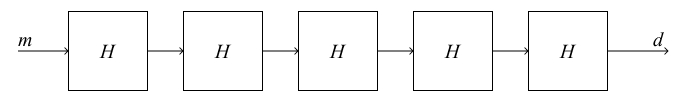
\includegraphics[width=1\textwidth]{Figures/background/hashchain_1.jpg}
  \caption[]{Example of a hash chain of length five.}
  \label{fig:hash-chain-1}
\end{figure}

This concept was proposed by Lamport as a way to securely store passwords on servers~\cite{hashchain}. In his proposed protocol, the server just stores $H^n(p)$, where $p$ is the password and $n$ is relatively big number (e.g. 1000). When the user wants to authenticate, she sends $H^{n-1}(p)$ and the server computes $H(H^{n-1}(p))$ and checks if it corresponds to $H^n(p)$. If this check succeeds, the user is authenticated and the server replaces the stored value with $H^{n-1}(p)$. Next time she wants to authenticate again, she needs to send $H^{n-2}(p)$ and this value is checked against the previously sent digest $H^{n-1}(p)$. In this protocol, even if the transmission or the storage is not secure, the password is safe.

Blockchain technology uses this idea to form the immutable chain of blocks: each block contains the hash of the previous one. Modifying a block would result in changing its hash, this would break the chain since all the following blocks would have to be recomputed, changing each digest. As shown in~\cref{fig:hash-chain-2}, it is a slightly different concept than the plain hash chain, since on each step, the hashing is done on the previous digest linked to raw data of the current block, so $d_{n}=H(b_n~||~d_{n-1})$

\begin{figure}[H]
  \centering
  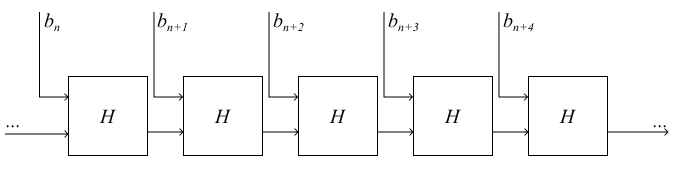
\includegraphics[width=1\textwidth]{Figures/background/hashchain_2.jpg}
  \caption[]{Example of how the hash chain concept is used in a blockchain.}
  \label{fig:hash-chain-2}
\end{figure}

\subsection{Merkle trees}

A Merkle tree is a data structure that generalizes the hash chain to efficiently prove membership of data. It is a binary tree in which each leaf node represents the hash of data, while intermediate nodes are computed as the hash of the two child nodes. \Cref{fig:merkle-tree} is an example of a Merkle tree with 4 leaf nodes.

\begin{figure}[H]
  \centering
  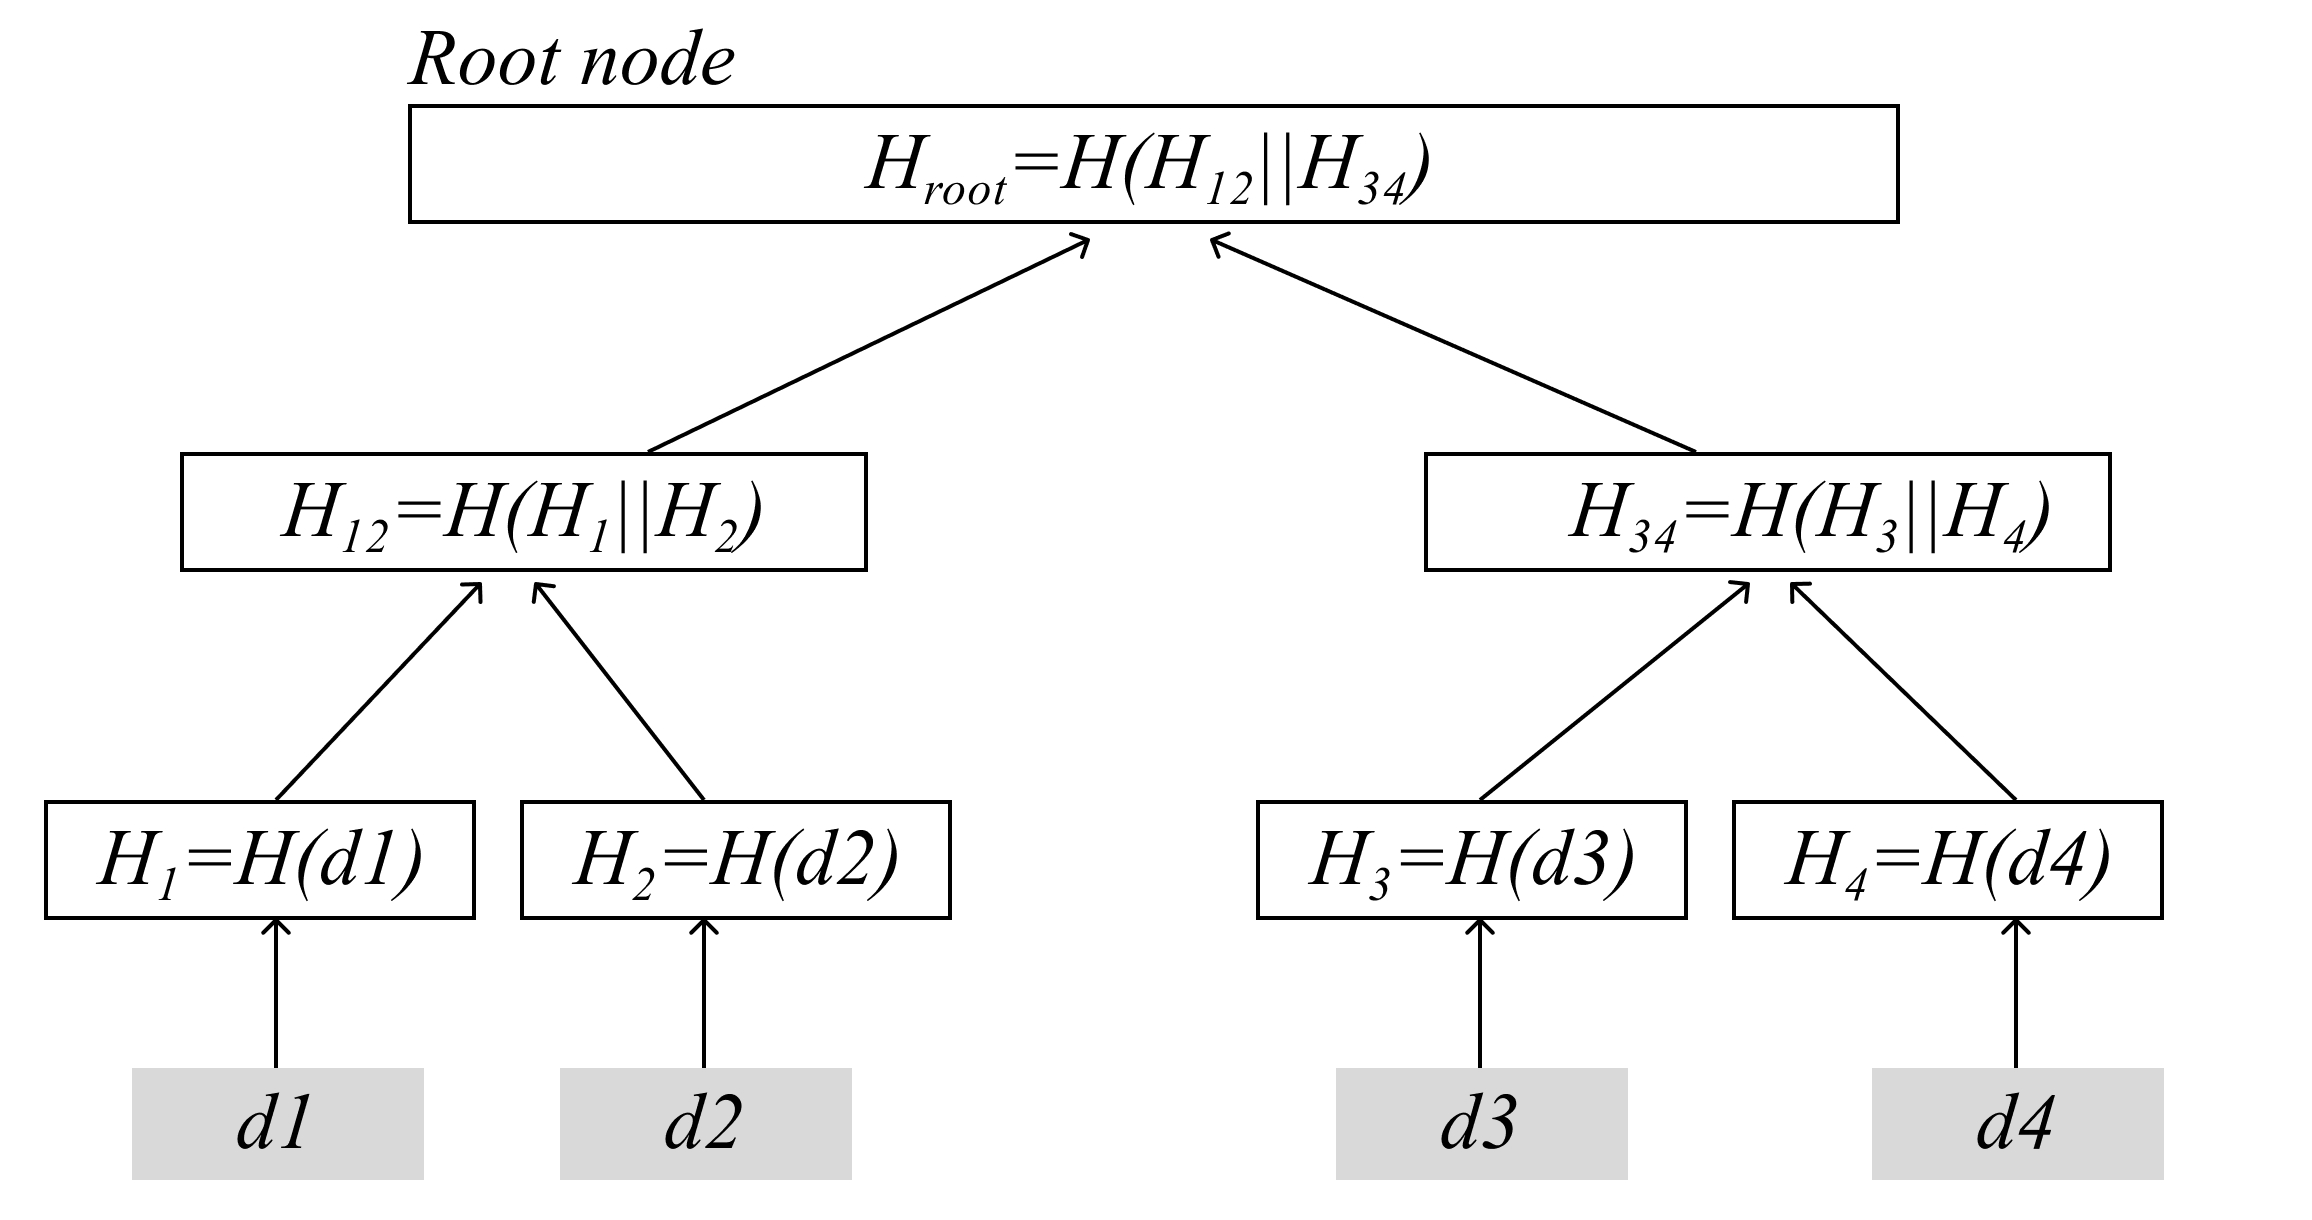
\includegraphics[width=1\textwidth]{Figures/background/merkle_tree.jpg}
  \caption[]{Example of a Merkle Tree with four leaf nodes.}
  \label{fig:merkle-tree}
\end{figure}

Proving membership of data to a tree with $2^n$ leaves just requires $n$ steps and $n$ intermediate nodes. The algorithm simply reconstructs the tree starting from the node that must be checked, recalculating again the root node, also called \textit{Merkle proof}. Data is proved to be part of the tree if the recalculated root node is equal to the given root node of the tree.

This exact concept is used in Bitcoin to prove membership of transactions to a block. Each block uses a Merkle tree where the leaf nodes are made by the hash of transactions. Inside each block it is stored the root of the Merkle tree. To prove that a particular transaction has been included in that block and not modified, it is necessary to rebuild the root node starting from the leaf of the transaction considered. This is particularly efficient for light clients. They do not store all the transactions, but just the block headers. If they need to prove that a certain transaction has been included in a block and not modified, they need to ask a full client just the intermediate hashes needed to rebuild the tree and not all the transactions of that block.

Ethereum uses a similar concept to store and verify membership of three different kind of information per block: 

\begin{itemize}
    \item State trie: it is a description of each account state used and modified at the current block.
    \item Transactions trie: similarly to Bitcoin, it describes each transaction included in the block.
    \item Receipts trie: it contains the receipts of the transactions included in the block.
\end{itemize}

All this data is stored in three different \textit{Merkle Patricia Tries}. It is similar to a plain Merkle tree but it is faster to edit, does not depend on the order of data and has a limited depth.

\subsection{Digital signatures}

A digital signature is the digital counterpart of a handwritten signature in the physical world. It uses asymmetric cryptography to securely prove that a certain entity created a piece of digital data and did not modify it since signing. 

This is achieved through the use of two keys:

\begin{itemize}
    \item \textbf{Private key}: it is a random sample of bytes used by the signer to sign messages and, as the name suggests, is kept secret.
    \item \textbf{Public key}: it is obtained from the private key and shared to the verifier to check if the signature is valid.
\end{itemize}

The process of signing a message $m$ works as follows:

\begin{enumerate}
    \item The signer calculates $d=H(m)$.
    \item The digest $d$ is encrypted using the private key resulting in the generation of the signature $\sigma$, that is included in the message to prove authenticity.
\end{enumerate}

To check if the signature is valid, the verifier needs the message $m$, the signature $\sigma$ and the public key of the signer. Anyone with this data can independently check that the signature is authentic and thus that the entity who owns the private key related to the signature is the creator of the message. 

There are multiple algorithms that make the public-key cryptography possible. In the sector of blockchain, the most used algorithm is \textbf{ECDSA}~\cite{ecdsa}. It is based on the discrete logarithm problem on elliptic curves over finite fields. On these curves, the problem of finding a $k$ such that $P=kG$, where $P$ is a known point on the curve and $G$ is a generator point, has an exponential complexity. 

Both in Bitcoin and in Ethereum, the addresses are obtained from ECDSA public keys in slightly different ways. Both networks use the same elliptic curve called \textit{secp256k1}.



\section{The blockchain}

The concept of blockchain was first introduced by the pseudonym Satoshi Nakamoto when he/them presented Bitcoin, back in 2008. It makes use of a p2p network and the previously cited cryptographic technologies to create a distributed digital ledger without the presence of a centralized authority. Blockchain refers to an abstract concept that is implemented in a lot of different protocols, but Bitcoin and Ethereum remain by far the two most important implementations.

In all the blockchains, the distributed ledger is represented in form of blocks secured together as a hashchain. Data can be added to this ledger by anyone trough transactions. To include a transaction in a block, and so to write to the ledger, users must send it to the p2p network and pay a fee. The payment is done trough a \textit{cryptocurrency} that has value just inside a specific network (e.g. Ether in Ethereum and Bitcoin in the Bitcoin network). The distributed ledger keeps track of the holdings of the cryptocurrency.

The consistency and the validity of what is written on the blockchain is based on the consensus. What is written in the ledger is correct if the majority of the people participating in the network agrees on it. There are multiple ways of achieving so that are discussed in the next sections, but all these methods share the fact that they are computationally not efficient. All the computers participating in the network must perform the same calculations in parallel to check the data they receive and eventually agree on its correctness. This is expensive since millions of computers are performing the same calculations instead of working on different tasks in parallel. 

This very inefficient computational pattern has become popular for the problem it solves: preventing double-spending without a central authority. 

\subsection{The double-spending problem}

In the world of digital payments, the double-spending problem refers to the possibility, by malicious actors, to use the same unit of value more than once. Given the nature of digital money or assets, it is very easy to duplicate them and use them multiple times.

The traditional and easy way of solving this problem is by introducing a central authority that controls all the transactions. To make a payment, users need to go trough a central authority that guarantees the validity of the transaction. The central authority stores internally a list of holdings. This solution introduces the bottleneck of having a single point of failure. The central authority must be always online, must always behave honestly and must guarantee the security of the data it stores. 

There were multiple historical attempts to remove, at least partially, this dependency from a central authority. A relevant attempt was ECash by David Chaum using RSA blind signatures in 1982~\cite{blind-signatures}. This protocol did not remove the concept of a central authority, but tried to reduce their power. Here the central authority, or bank, issues coins to users signing them with blind signatures. The peculiarity of this type of signature is that the signer does not know the message it is signing, so the coins are anonymous and untraceable. Users can send these digital coins between each other even if the bank is offline. The receiver then proceeds to send these coins to the bank to deposit the money into his bank account. In this protocol, double spending is prevented completely just if the bank is online but can also be detected offline if the same coin is sent multiple times to the same receiver.

In the concept of blockchain this problem is solved by letting all the participants of the network know and agree on who owns what and which transactions are taking place. If a user tries to submit a transaction that is spending money that she had already spent, the other participants of the network will not agree on including it into the blockchain and the money transfer will never occur.

For technical reasons it would be possible to encounter double spending also in blockchain transactions due to temporary forks. It is a situation in which there are two new blocks to include on the top of the chain at the exact same moment. This event will result in having two different chains, both valid. The blockchain protocols usually work in a way to always follow the longest available chain, so it is necessary to wait for the inclusion of new blocks and see which of the available chains outgrows the others. This is the reason why in blockchain transactions it is needed to wait for confirmations. A common heuristic in Bitcoin is to wait for 6 new blocks to be added on top of the desired one to be sure that it is final, this means waiting for around one hour. In Ethereum, with the recent migration to Proof of Stake, it is required a maximum of around 15 minutes to be sure that a block is finalized and can not be replaced.

\subsection{Blockchain properties}

The word blockchain is often accompanied with many adjectives to describe its properties. I here try to summarize and explain the most common ones:

\begin{itemize}
    \item \textbf{Decentralized}: there is not a central authority that rule and control the network. No-one in the network has the power to control or change the rules. All the actors follow the protocol and have the same power.
    \item \textbf{Distributed}: the computation is performed by multiple distinct computers that interacts with each other through a p2p network. The failure of a machine does not interrupt the protocol.
    \item \textbf{Immutable}: it is not possible to alter the history of what has been written on the blockchain. Once a block is included and finalized it is not possible to modify it.
    \item \textbf{Permissionless}: everyone can actively participate in all the roles of the network without asking for permissions.
    \item \textbf{Permissioned}: in contrast to permissionless, permissioned blockchains requires that the actors receive explicit authorization to operate on the network. The most used example of this kind is Hyperledger Fabric\footnote{Hyperledger Fabric is a modular framework for enterprise blockchains: \url{https://www.hyperledger.org/projects/fabric}.}.
    \item \textbf{Transparent}: everyone can independently download and read blockchain data. The only things needed are a computer and an internet connection. It is possible to get the data using specific software called clients, that are specific for each protocol.
    \item \textbf{Pseudoanonymous}: users that participate in the network does not need to prove their real identity. Every activity on the chain is linked to an address and not to a real person. 
    \item \textbf{Account-based}: data is saved based on account. Each account has a balance that can be spent. In order to spend this balance, users need to prove they have a private key related to the account's address.
    \item \textbf{UTXO-based}: contrary to account-based blockchains, the model of UTXO just has the concept of transactions. Users need to prove they have the private key for unlocking the output of a transaction to spend its money. The balance of a user is simply the sum of the values of the outputs he can potentially unlock and spend.
\end{itemize}

\subsection{Consensus layer}

As said in the previous sections, the fundamental concept in the blockchain technology is that the validity of the data stored is based on the consensus between the majority of the actors participating in the network. This section explains how this is achieved trough different types of \textit{consensus layer}.

All public blockchains need to have a consensus layer to make the users agree on what is correct. There are many different types that have been invented in the years, but the two most important layers are \textit{Proof of Work (PoW)} and \textit{Proof of Stake (PoS)}.

\subsubsection{Proof of Work}

The Proof of Work consensus mechanism is the one introduced with Bitcoin back in 2008. It has been used also by Ethereum until the switch to Proof of Stake happened in September 2022. 

The core concept in Proof of Work is that users need to solve complicated \textit{puzzles} in order to write data on the blockchain. The solution to the puzzle shows that the user who found it has performed a lot of work and grants him the permission to write on the chain. All the other actors, that were not able to solve the puzzle, limit themselves to check the validity of the solution.

The PoW layer has a mechanism to algorithmically adjust the difficulty of the puzzles. Each blockchain protocol sets a fixed amount of time in between blocks, called inter-block time. In case of Bitcoin it is of 10 minutes. If the solutions to the puzzles are found faster than the expected inter-block time, the next puzzles will become more complicated. On the other hand, if the inter-block time is higher than the expected one, the following puzzles will be easier to solve.

The puzzle that must be solved in Bitcoin is the following: find a (double) hash of the data contained in the block's header such that is is lower than a threshold that depends on the current difficulty. It can be summarised as the following equation: $H(H(header)) < $ \textit{difficulty threshold}. The output of a hash function is a fixed amount of bits, so it can also be said that the puzzle is finding a digest that starts with a certain amount of zeros (and so that is a small number).

There is a field in block headers called \textit{nonce} that is used for solving these puzzles. It is a 32 bits fields that can be freely set by the \textit{miners} to cause the hash to change and meet the requirements of the puzzle.

The word \textit{miner} comes from this concept. The users that try to find the solution to the challenge are called miners since they continuously try to find valid hashes that would provide them a precious reward. 

Miners are economically incentivized to perform the hard work of mining since they receive a reward for each block mined and also all the transaction fees of the transactions included in the mined block.

In Bitcoin, these are the steps to follow to mine a block with PoW:

\begin{enumerate}
    \item Choose the block's content. Include transactions, coinbase transaction and compute the Merkle root.
    \item Choose a random 32 bit nonce and include it in the block's header.
    \item Compute the double hash of the block's header. If the result is lower than the difficulty target the block is successfully mined. If not (and not all nonces has been tried), go to step 2.
    \item If all nonces has been tried, go back to step 1. 
\end{enumerate}

PoW has proven to work well with Bitcoin, but it suffers of some limitations:

\begin{itemize}
    \item High energy consumption: Bitcoin alone is estimated to use around 45.8 TWh per year for running the computers that perform mining. This is between the levels produced by the nations of Jordan and Sri Lanka~\cite{bitcoin-footprint}.
    \item Risks of centralization: the hardware used for mining is becoming more and more expensive and it is a big entry barrier for small players. There is the risk that few big players together can take control of the blockchain. This happened in 2014, when the GHash.io mining pool had more than 51\% of the hashing power of Bitcoin.
\end{itemize}

\subsubsection{Proof of Stake}

Proof of Stake is the most popular alternative introduced to reduce the drawbacks of Proof of Work. Here, the permission to append data to the blockchain is granted randomly between a set of \textit{validators}. 

To become a validator, a normal user has to \textit{stake} a certain amount of coins. These coins are kept locked in a smart contract and can be used by the protocol as a warranty that the validator will behave correctly. If the validator fails to do his work, the coins staked can be \textit{slashed}, like a fine to disincentive bad behaviours.

The idea is that miners, instead of spending money in computers and energy, spend their money by locking the coins. This has the advantage of not wasting energy and also gives more value to the coins themselves.

The most popular blockchain that uses this consensus layer is Ethereum. It switched from Proof of Work to Proof of Stake in September 2022, reducing emissions from 78 TWh/yr to just 0.0026 TWh/yr\footnote{More details about this can be found on the Ethereum website: \url{https://ethereum.org/en/energy-consumption/}.}. In Ethereum, users are required to stake 32 ETH, equivalent to 52,402 USD, to become validators.

\subsection{51\% attack}

The 51\% attack is the nature consequence of how the blockchain works. Everything is based on consensus, this attack simply gains the majority of it. It consists in the case in which a single entity owns more than half of the hashing power (in case of PoW) or more than half of the staked coins (in case of PoS). 

In these cases, this single entity has the control of more than half of the network. In case of PoW, he can mine block faster that anyone else and so he can create a fork that will outgrow the current chain that in the meantime can be used to double spend money. In case of PoS, he has the control of the majority of attestations, so he can vote his own fork to be the preferred fork and again double spend money.

The security of a blockchain against the 51\% attack is related to how much it would cost to perform such an attack. It would cost billions of dollars to buy the infrastructure to perform a 51\% attack against Bitcoin. The more a blockchain is used and the more it is secure against 51\% attacks. 

\section{Ethereum}

Ethereum is a decentralized, permissionless and account-based blockchain. It is the second blockchain in terms of market capitalization\footnote{Market capitalization refers to the total value of all the cryptocurrency emitted.} and popularity. It was designed and developed by Vitalik Buterin and Gavin Wood since 2013. It went live in 2015. It was the first of many \textit{Blockchain 2.0}, so a blockchain that allows users to create smart contracts using a Turing-complete programming language.

It was introduced to generalize the potentiality of the blockchain technology and make it available to other use cases than just money transfers. Thanks to the Turing-complete scripting language, it is possible to create applications that can implement any kind of logic that could benefit of a blockchain. Previously to Ethereum, it was common to create ad-hoc protocols for each use case. This created fragmentation and caused low adoption. 

As stated by Vitalin Buterin in the announce post on the Bitcoin forum\footnote{The thread can be found at the following link: \url{https://bitcointalk.org/index.php?topic=428589.0}}, the goal of Ethereum was to "to provide a platform for decentralized applications - an android of the cryptocurrency world, where all efforts can share a common set of APIs, trustless interactions and no compromises". 

\subsection{Ethereum as a state machine}

The Ethereum blockchain can be seen as a state machine. There is a global state, called \textit{World State}, that stores data related to each ever-used account. This state is modified trough transactions, after their inclusion in each block. \cref{fig:ethereum-state-machine} visualizes this concept clearly.

\begin{figure}[H]
    \centering
    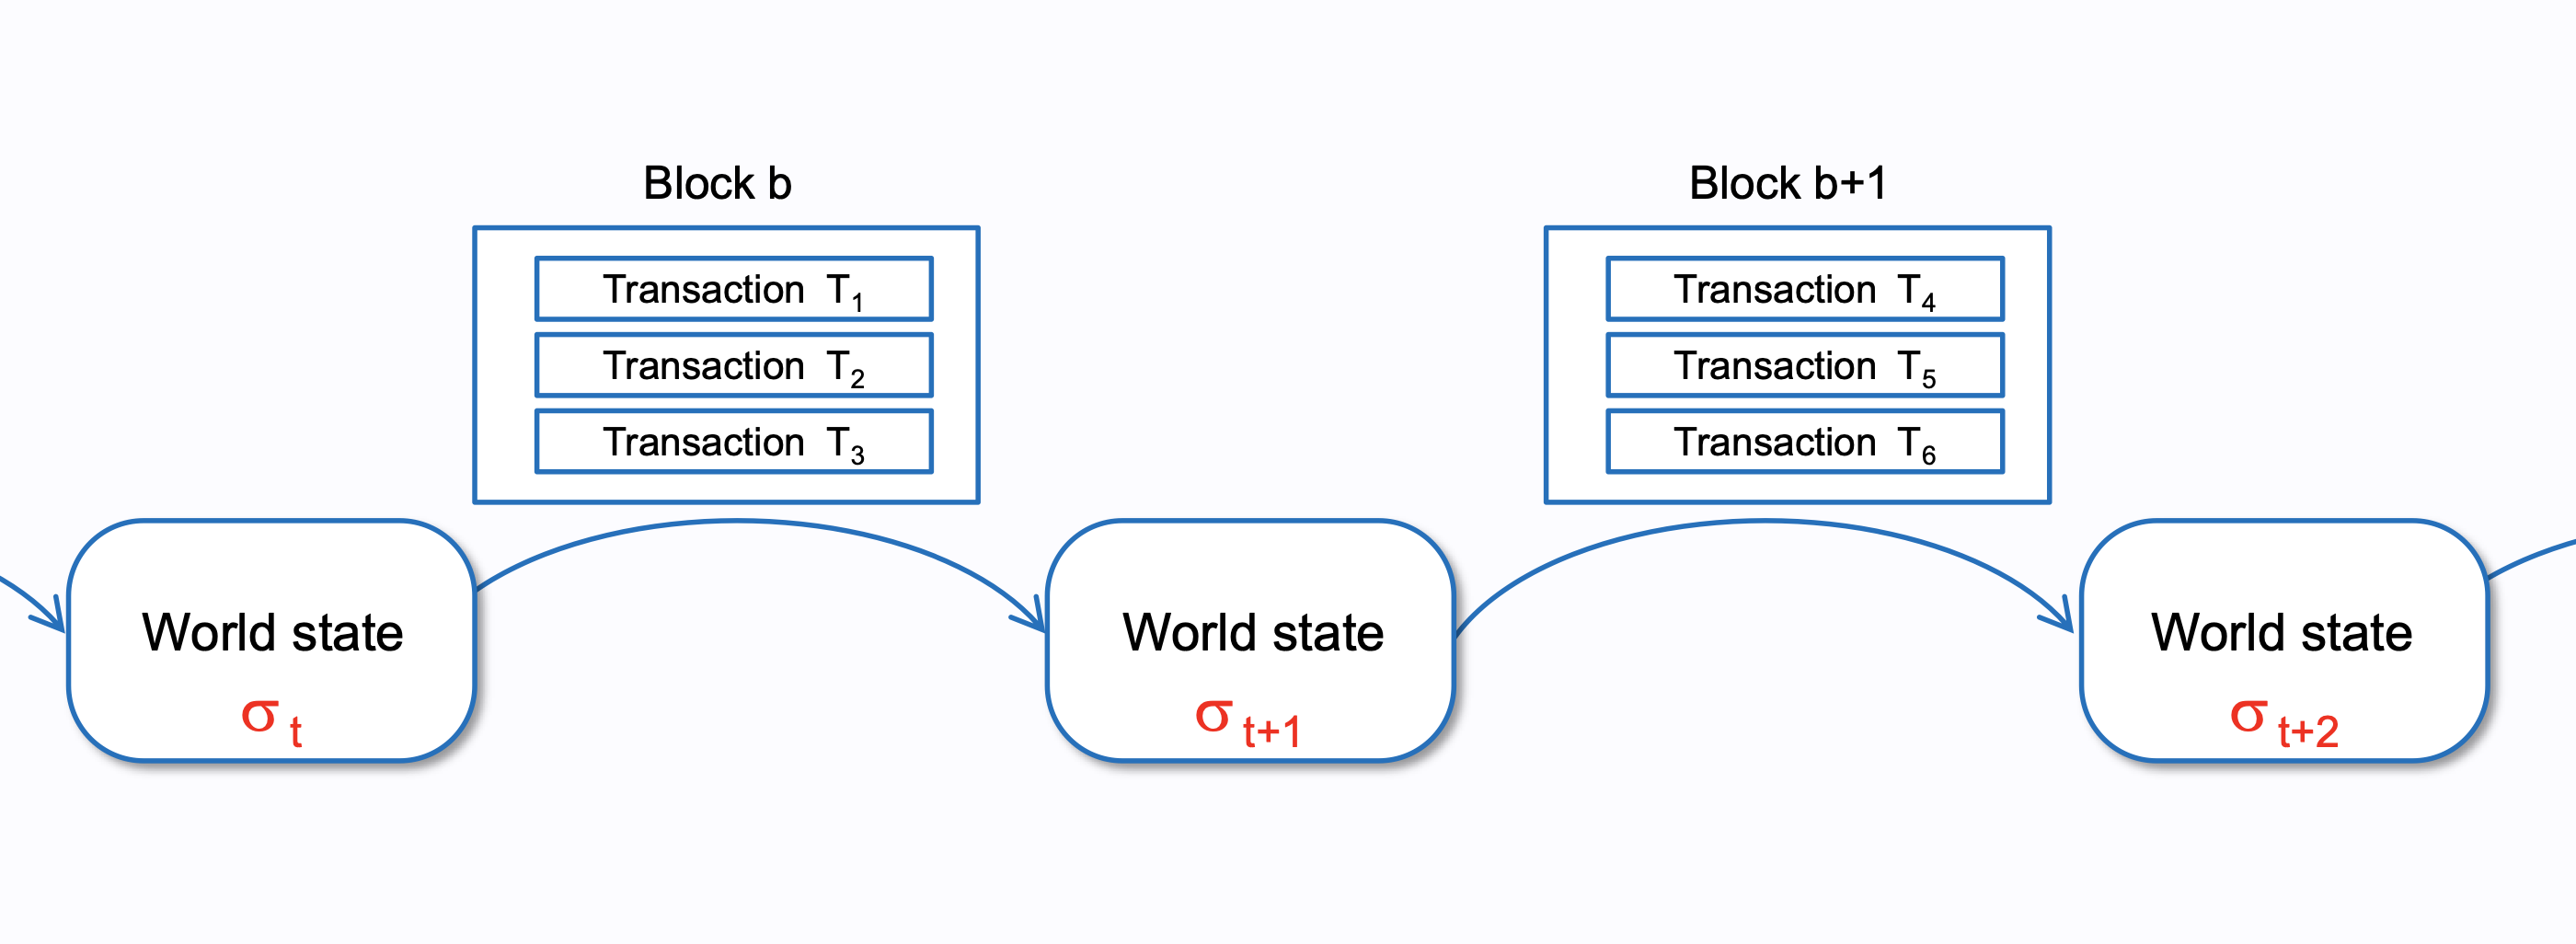
\includegraphics[width=1\textwidth]{Figures/background/state-machine.png}
    \caption{Ethereum visualized as a state machine~\cite{evm-illustrated}.}
    \label{fig:ethereum-state-machine}
\end{figure}

The World State is a mapping between account address and account state. There are two types of account: Externally Owned Account (EOA) and Contract Account (CA). EOA is the traditional account based on a private key, used to generate transaction on the chain. It needs to store on the World State just two pieces of data: a nonce and its balance. The Contract Account refers to smart contracts, they can not generate transactions, they can just react to them. On top of nonce and balance, it needs to store on the World State also the storage hash and the code hash. These two hashes are used as pointers to retrieve the storage of the smart contract, so the place in which the software stores variable values, and the actual code to run when invoked from a transaction. \Cref{fig:ethereum-world-state} shows the division of the World State.

\begin{figure}[H]
    \centering
    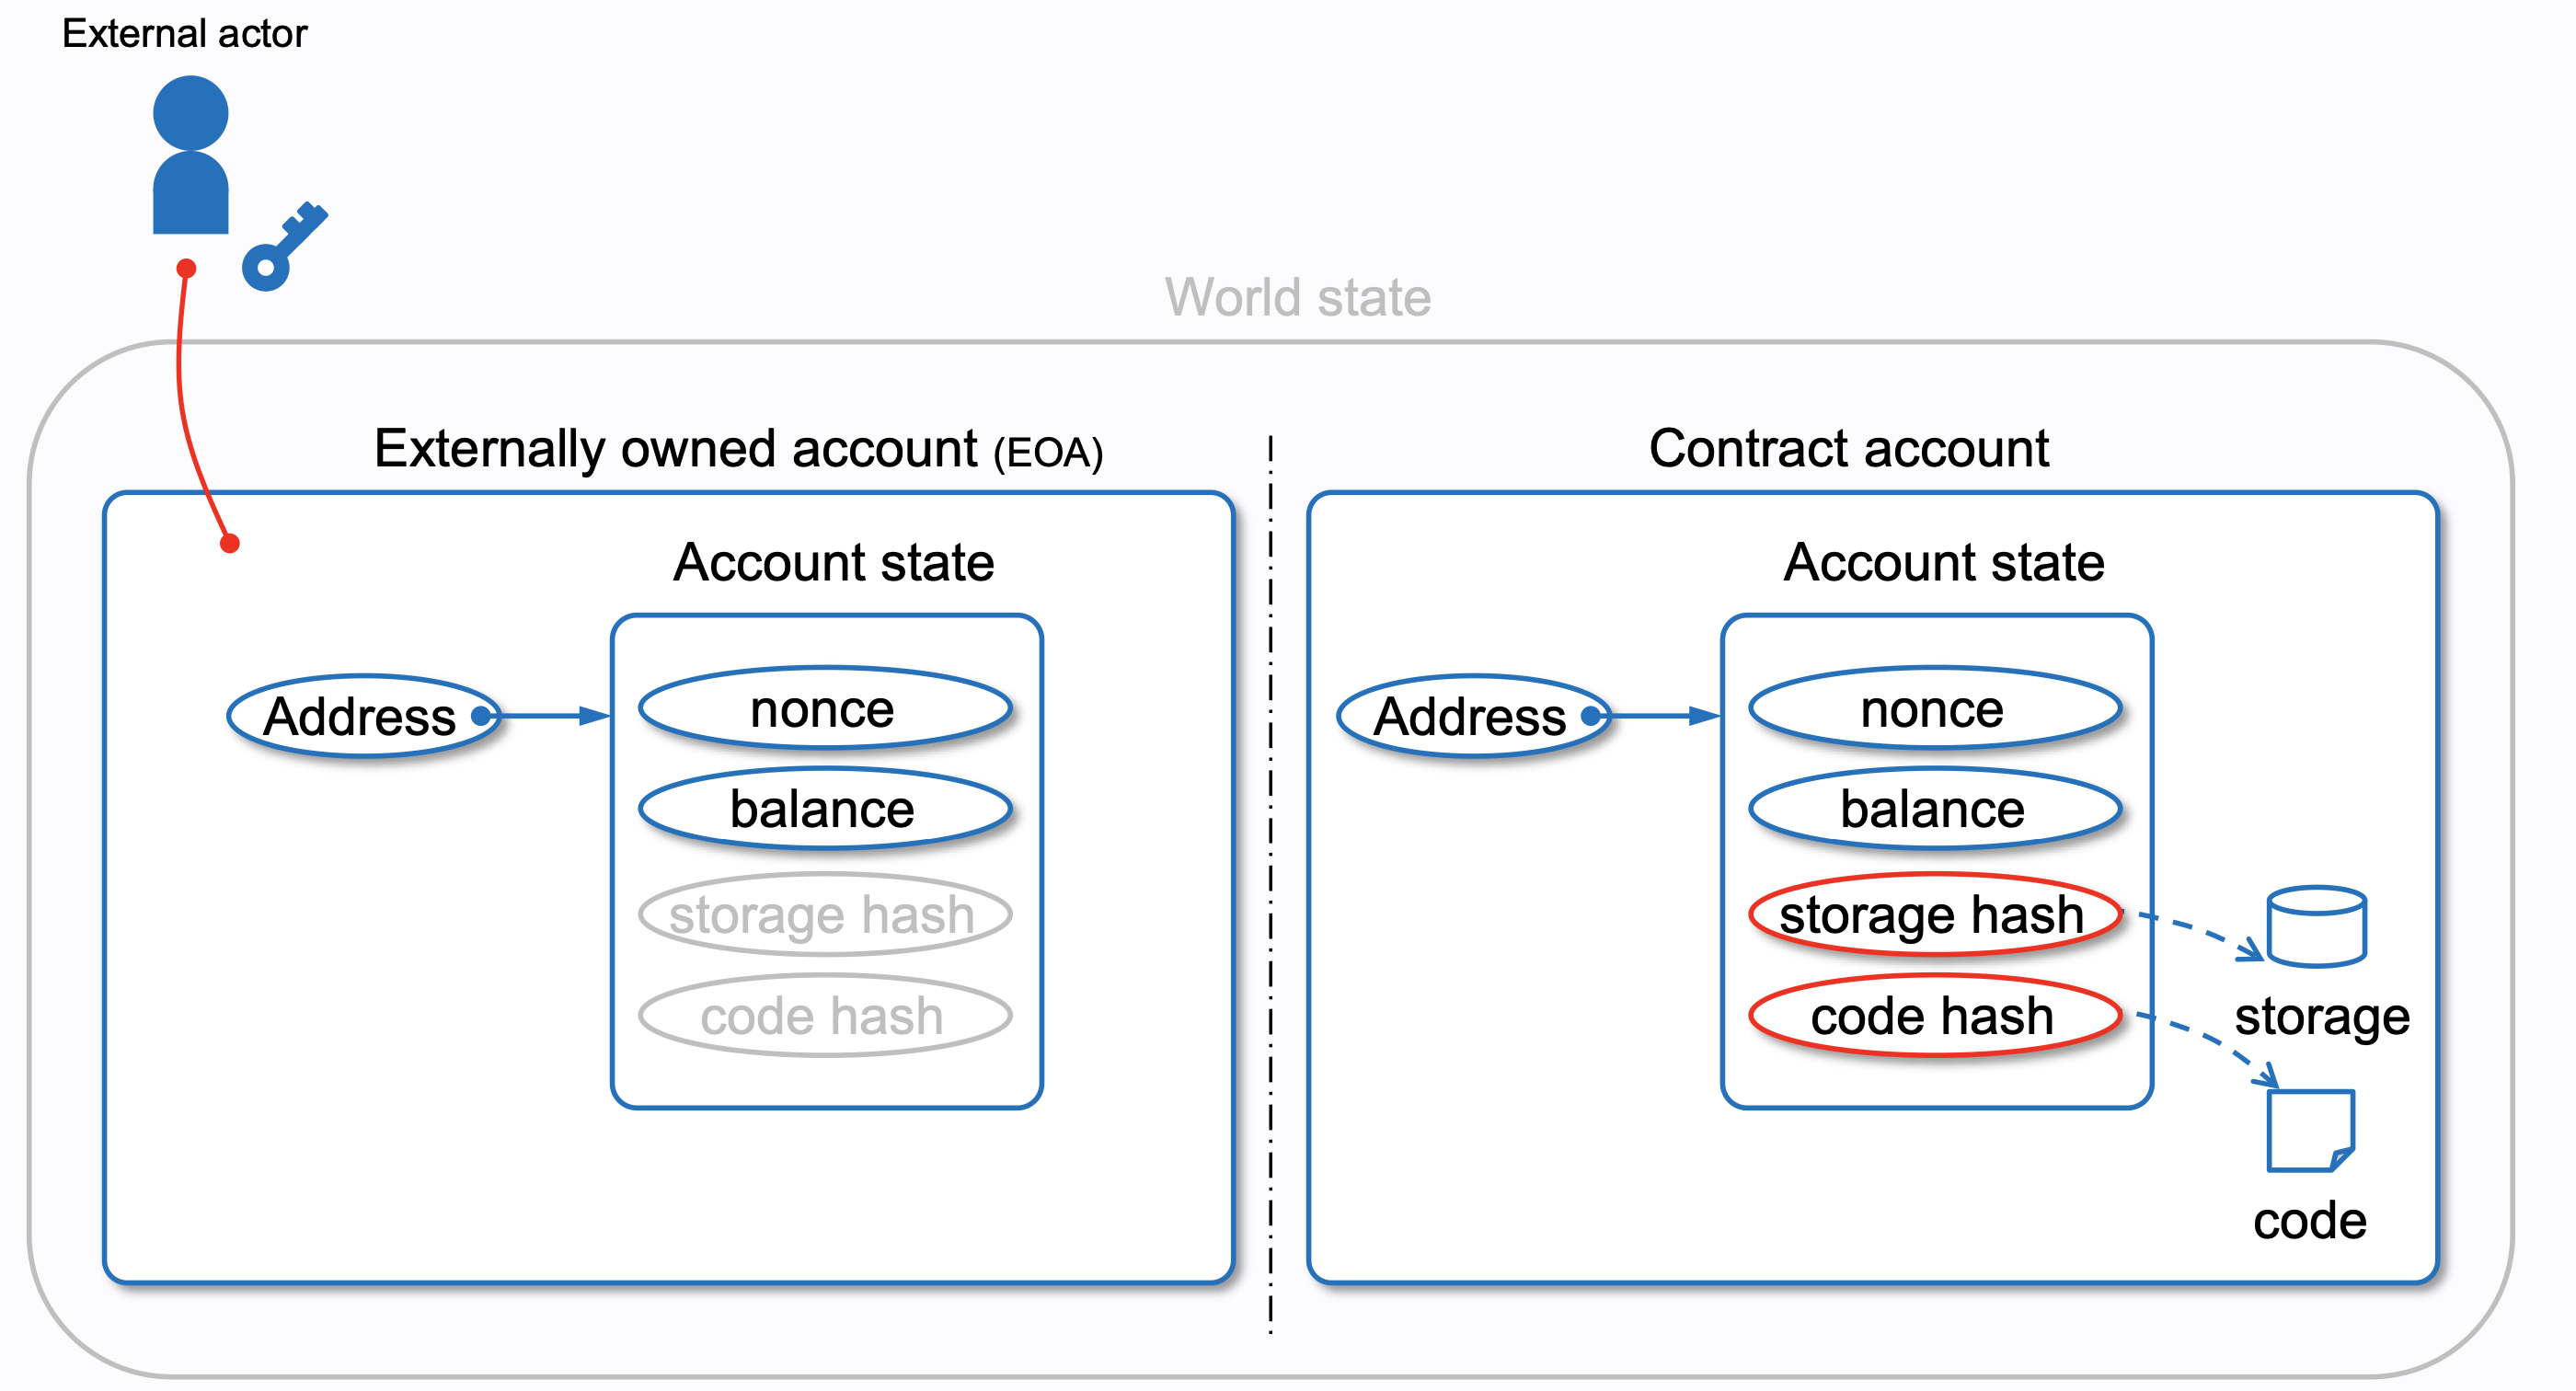
\includegraphics[width=1\textwidth]{Figures/background/world-state.png}
    \caption{Ethereum World State visualized~\cite{evm-illustrated}.}
    \label{fig:ethereum-world-state}
\end{figure}

This World State needs to describe the state of millions of accounts and update it every 12 seconds, the average inter-block time in Ethereum. To do so, it uses a Merkle Patricia Trie that is optimized for this use case. 

\subsection{Ethereum Smart Contracts}

Smart contracts are pieces of code that can be invoked trough transactions and that can modify the World State following a custom logic. They are written in high-level programming languages compiled to a stack-based bytecode called {\tt Ethereum Virtual Machine code} or {\tt EVM code}. 

Smart contracts can do many things, such as:

\begin{itemize}
    \item Store data on the blockchain: each smart contract has a storage in which it can store persistent data represented by \textit{state variables}. Storing persistent data has a cost and is paid through \textit{gas}.
    \item Interact with other smart contracts: during its execution, a smart contract can call other smart contracts and use their return values.
    \item Emit events that are indexed: it is possible to use the \lstinline{LOG} opcode to store persistent data that is indexed by the Ethereum clients. This indexed data can be easily retrieved by traditional software through fast RPC calls. 
    \item They can handle failures: it is possible for a smart contract to gracefully handle failures both totally or partially. Everything that is done in a failed branch of a transaction is not persistently stored on the blockchain.
    \item Access context data: it is is possible to access block and transaction data inside the execution of the code. It is very common to use the address of the transaction's sender to manage access to certain restricted functions.
\end{itemize}

But at the same time, smart contracts on Ethereum have some limitations that limit their applicability to real-world scenarios:

\begin{itemize}
    \item No access to external data: from the code of a smart contract it is impossible to know everything that is outside of the blockchain. It is not possible to call a REST API to get information such as stock prices, weather or any other data. This is partly solved by \textit{oracles}, that are specific smart contracts that can be queried to get these kind of information. These smart contracts are updated by transactions sent periodically by an external entity. It is an expensive operation and creates a potential single point of failure.
    \item Cannot connect to any other software: as said before, it is not possible for a smart contract to interact with other software that are not other smart contracts on the same chain. The link between traditional systems and smart contracts is always asynchronous, e.g. they can not cooperate during the execution of a transaction.
    \item No infinite loops: smart contracts can not execute endless loops. This is an obvious limitation, since the execution of a transaction must finish in order to include its outcomes in the World State.
    \item Hard to upgrade: it is not possible to change the code of a smart contract once it is deployed on the blockchain. There are some ways of doing it as explained in \cref{chapter-analysis} but it is not trivial. 
    \item Cannot initiate transactions: smart contracts are passive entities on the blockchain that can be invoked by external users. They can not create transactions by their own.
    \item Cannot accept randomness: the execution of a smart contract must be completely deterministic. It must be reproduced on each node participating in the network to attest its correct execution and so it can not accept any real randomness.
    \item  Cannot store sensitive or private data: since Ethereum is a permissionless blockchain, everything stored there is public. Smart contracts can not hide anything. 
\end{itemize}

\subsubsection{Gas}

The concept of gas has been introduced in Ethereum to have a unit of measure for pricing smart contract executions. Miners involved in the protocol must run the smart contracts' code on their machines to calculate the World State differences. Malicious users could potentially send computationally intense transactions to congest the network. This is avoided in Ethereum using gas, which makes this kind of attack economically not convenient.

Each EVM opcode has an associated price that indicates how much gas it burns when it is executed. The amount of gas each transaction can burn is finite, so it is impossible to encounter infinite loops. If a user tries to code an infinite loop or even just an expensive code execution, the transactions will fail with the error \textit{out of gas}.

Ethereum gas has a variable price that changes based on the congestion of the network. It is paid in Ethers by the sender of the transaction. Before EIP-1159\footnote{EIP-1159 is an Ethereum Improvement Proposal that changed the fee market. It can be read here: \url{https://eips.ethereum.org/EIPS/eip-1559}.}, the price of gas was set by each user when he built the transaction. The fee that the transaction sender had to pay was simply $gasPrice * gasUsed$. Transactions with higher \textit{gasPrice} were prioritized by miners since they rewarded more money for the same computational effort.

After EIP-1159, since August 2021, the gas fee has been split into two parts: \textit{base fee} and \textit{priority fee}. The \textit{base fee} is a gas price calculated by the network based on congestion. The \textit{priority fee} is an additional value given per unit of gas used to incentivize miners to include a specific transaction. For each transaction, $baseFee*gasUsed$ Wei\footnote{Wei is a fraction of a Ether. 1 Wei is $10^{-18}$ ETH.} are burnt and $priorityFee*gasUsed$ Wei are given to the miner.

\subsubsection{EVM}

EVM stands for Ethereum Virtual Machine and is the virtual architecture of the computer that runs the smart contracts' bytecode. The EVM is a stack based machine composed of a stack, a volatile memory and a program counter. It can access the World State both to read and to write persistent data. \cref{fig:evm-architecture} shows the schema of the EVM.

The whole Ethereum network can be seen as a single instance of an EVM machine that runs the code of smart contracts invoked in transactions. In practice, this is done by every single node connected to the network, using a potentially different EVM implementation.

\begin{figure}[!ht]
    \centering
    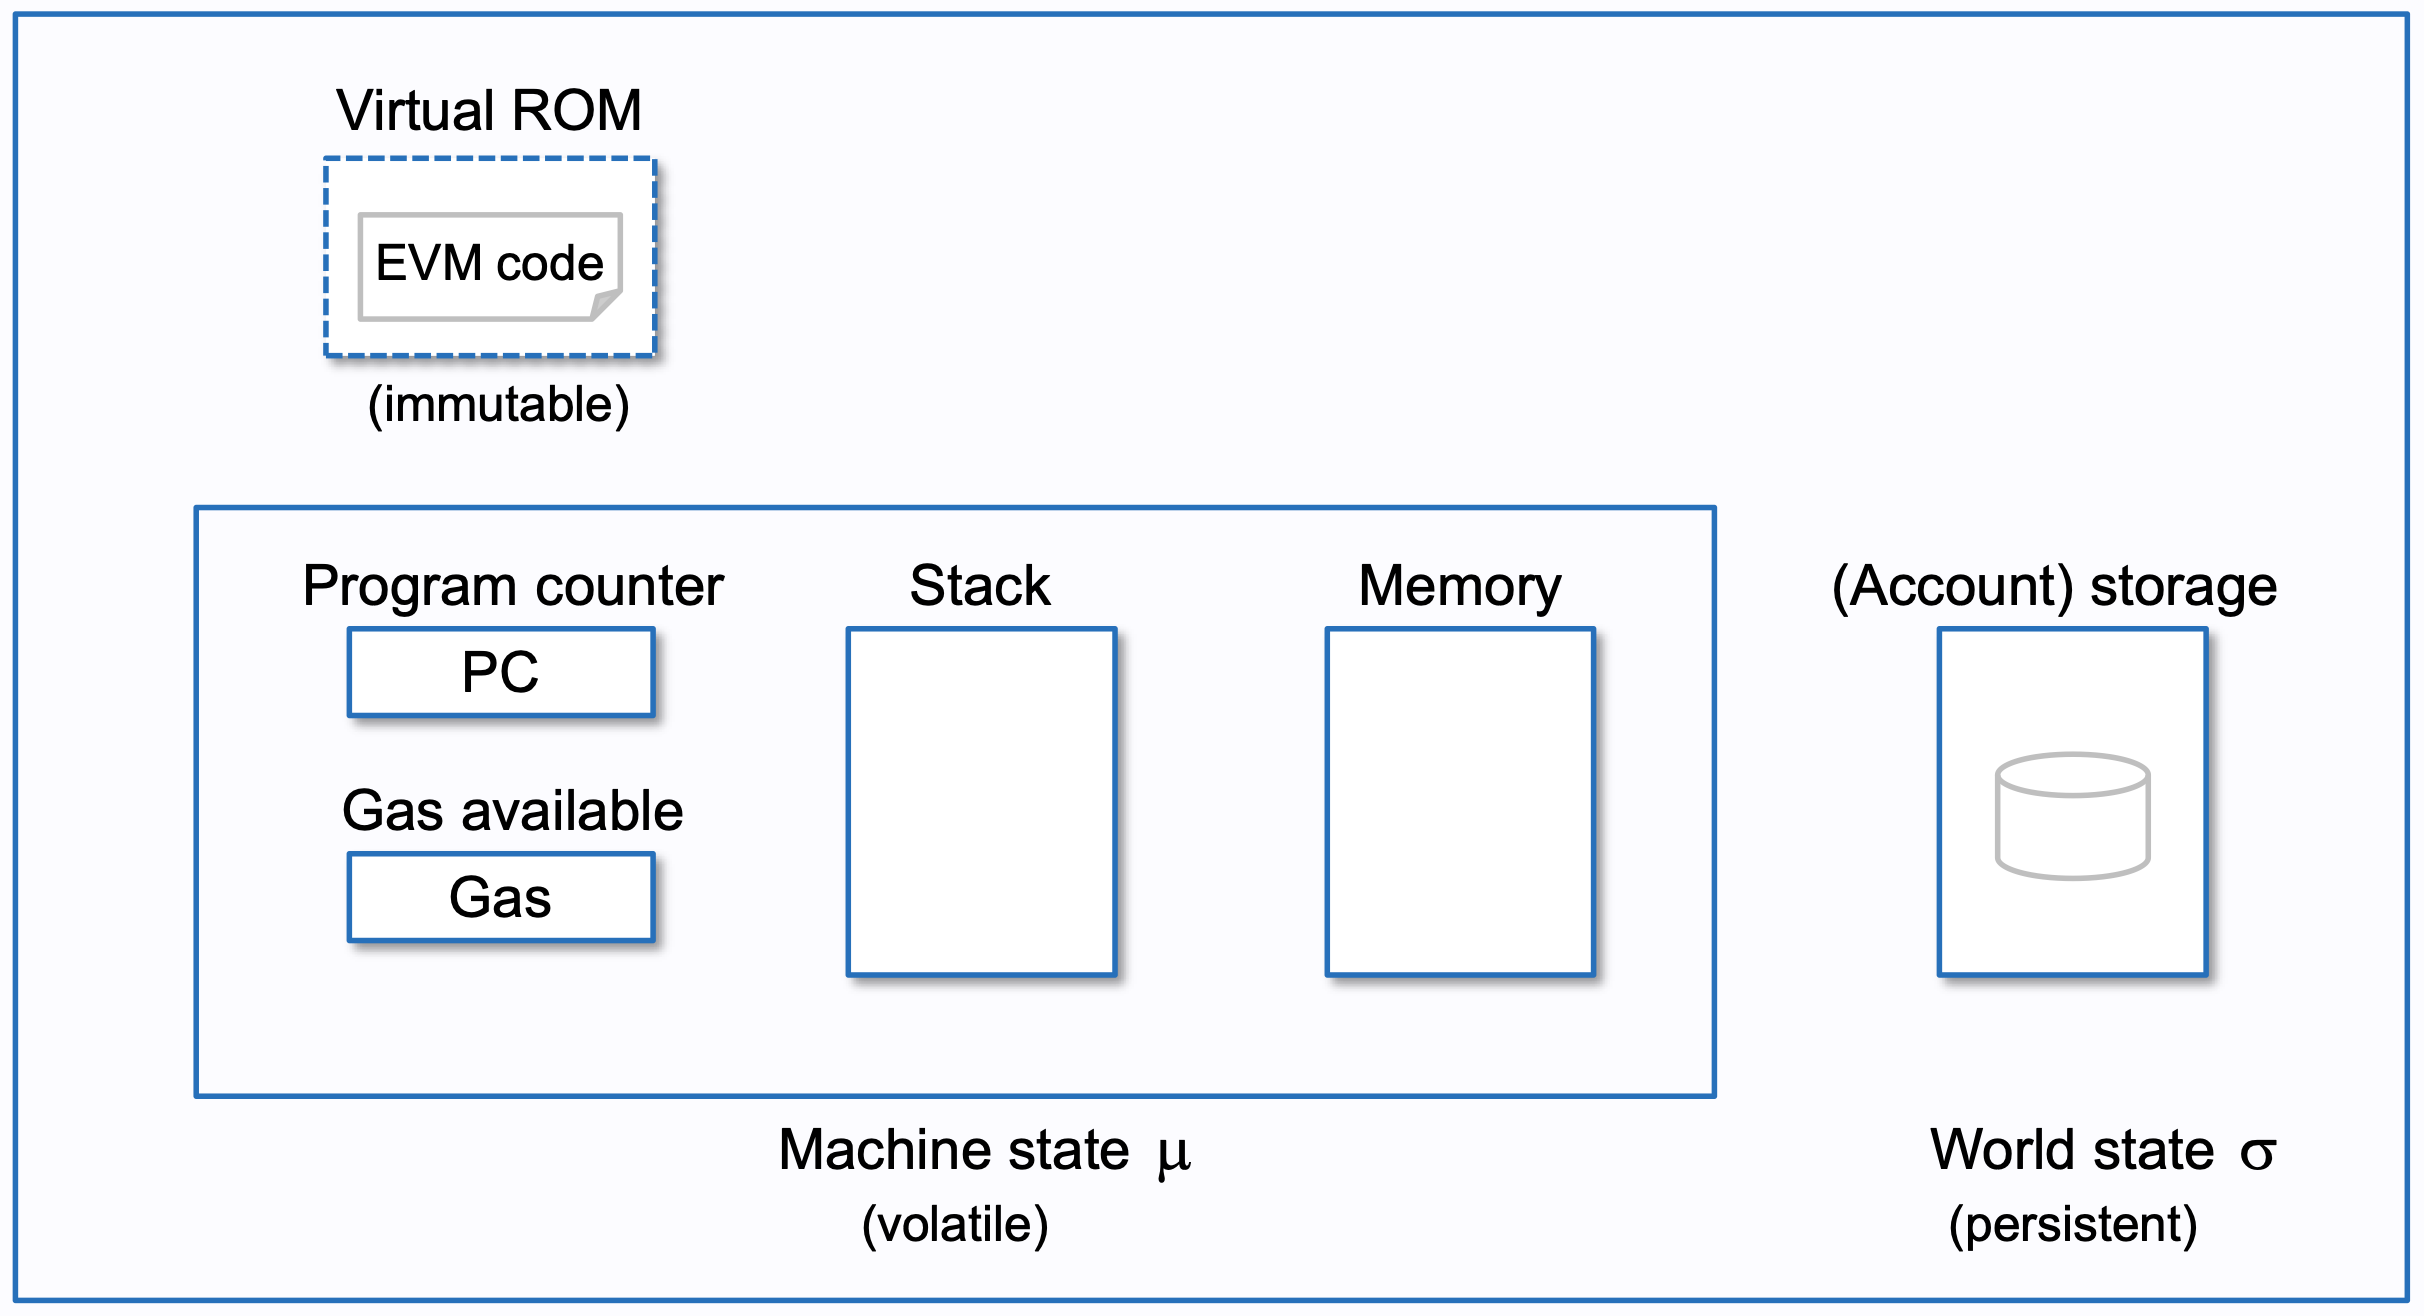
\includegraphics[width=1\textwidth]{Figures/background/evm.png}
    \caption{The Architecture of the Ethereum Virtual Machine (EVM)~\cite{evm-illustrated}.}
    \label{fig:evm-architecture}
\end{figure}

\subsubsection{Solidity}

Ethereum smart contracts can be programmed in many high-level programming language. Historically, two languages have been relevantly used: Viper and Solidity. Nowadays almost every smart contract is developed in Solidity, it is by far the most common language used for this purpose.

Solidity is a statically-typed programming language. The syntax is very similar to popular languages such as JavaScript. It works like an object oriented language: a contract is defined as a class that has a constructor and public or private attributes and methods.

It is compiled to EVM bytecode using \textit{solc}, a compiler written in C++. After the compilation with the \lstinline{--bin} flag, solc produces as an output the EVM bytecode that can be deployed to the Ethereum blockchain.

This bytecode includes both the runtime code and the deployment code. The first one is the actual code that is stored on the chain, while the second part is the code needed to initialise the contract. \cref{lst:solidity-example} shows an example of a basic smart contract taken from the Ethereum documentation. \cref{lst:solc-result} shows the result of the compilation of this contract. These are the 541 bytes that implement the logic of the Solidity code and that are stored on the blockchain.

\begin{lstlisting}[caption={Example of a simple Solidity smart contract that stores a variable on the blockchain and allows edits to it.},label={lst:solidity-example},captionpos=b, style=boxed]
// SPDX-License-Identifier: MIT
pragma solidity ^0.8.20;

contract SimpleStorage {
    // State variable to store a number
    uint public num;

    constructor(uint _num) {
        num = _num;
    }

    // You need to send a transaction to write to a state variable.
    function set(uint _num) public {
        num = _num;
    }

    // You can read from a state variable without sending a transaction.
    function get() public view returns (uint) {
        return num;
    }
}
\end{lstlisting}

\begin{lstlisting}[caption={EVM bytecode derived from compiling the contract shown in \cref{lst:solidity-example}. There are three parts divided by two underscores (\_\_). The first part is the deployment code, the second part is the runtime code and the last part is the CBOR-endoded metadata. This is what is stored on the blockchain and what can be retrieved.},label={lst:solc-result},captionpos=b, style=boxed,breaklines]
0x608060405234801561000f575f80fd5b5060405161021d38038061021d83
398181016040528101906100319190610074565b805f819055505061009f56
5b5f80fd5b5f819050919050565b61005381610041565b811461005d575f80
fd5b50565b5f8151905061006e8161004a565b92915050565b5f6020828403
12156100895761008861003d565b5b5f61009684828501610060565b915050
92915050565b610171806100ac5f395ff3fe__608060405234801561000f57
5f80fd5b506004361061003f575f3560e01c80634e70b1dc14610043578063
60fe47b1146100615780636d4ce63c1461007d575b5f80fd5b61004b61009b
565b60405161005891906100c9565b60405180910390f35b61007b60048036
038101906100769190610110565b6100a0565b005b6100856100a9565b6040
5161009291906100c9565b60405180910390f35b5f5481565b805f81905550
50565b5f8054905090565b5f819050919050565b6100c3816100b1565b8252
5050565b5f6020820190506100dc5f8301846100ba565b92915050565b5f80
fd5b6100ef816100b1565b81146100f9575f80fd5b50565b5f813590506101
0a816100e6565b92915050565b5f60208284031215610125576101246100e2
565b5b5f610132848285016100fc565b9150509291505056__fea264697066
7358221220ed271d25e577fb9fa9b0b77e93485c035d8fc87f28d3c0247cff
80d69910e46064736f6c63430008150033
\end{lstlisting}

\subsubsection{Token contracts, ERC20 and ERC721 standards}

The most frequent use case of smart contracts are tokens. Tokens can be of two types: fungible or non-fungible. Fungible tokens are divisible, like money, while non-fungible tokens can not be split, like a piece of art. 

At low level, fungible tokens are simply a mapping from account to the balance of the token that the account can spend. Non-fungible tokens, on the opposite, are simply a mapping from the token id to its owner. Those mappings are stored on the blockchain, and specific functions allow the owners of the tokens to transfer them.

Since the usage of tokens was so popular, the Ethereum community standardized them in two standards: ERC20\footnote{Link to the EIP-20 official page: \url{https://eips.ethereum.org/EIPS/eip-20}.}, for fungible tokens, and ERC-721\footnote{Link to the ERC-721 official page: \url{https://eips.ethereum.org/EIPS/eip-721}.} for non-fungible tokens. 

ERC20 specifies nine functions and two events that allows users to transfer their tokens or allow other users to spend them. Famous ERC20 smart contracts are stable coins (e.g. USDT, USDC) or DAO tokens (e.g. Uniswap, Lido DAO, Aave).

The same applies to ERC721, which specifies nine functions and three events that allows users to safely manage their non-fungible tokens. Popular ERC721 tokens includes CryptoPunks, CryptoKitties and the Ethereum Name Service.

The usage of standards allows developers to build applications that can interact with any token. For example, it is possible to develop decentralized exchanges and wallets that work with any smart contract that correctly implements one of the two standards.


\subsection{Ethereum clients}

Ethereum is just a definition of a protocol. It defines in details how participants of the network must behave. All the logic is implemented by complex software called \textit{clients}. A computer that runs a client and is connected to the network is called an \textit{Ethereum node}.

There are multiple different practical implementations of the Ethereum protocol, all the different kind of software interact with each other thanks to the protocol definition. It is actually very important for the network to have a diversity of the type of clients running simultaneously. This ensures that the network will still work in case a specific client receives a wrong update. Imagine the scenario in which there is only one client version in all the network and it receives a wrong update. The blockchain would stop to work correctly and it would be very hard to bring it back up with the correct state.

After the switch to PoS, clients are divided into two: execution and consensus clients. The execution client is responsible for managing transactions, executing smart contracts and updating the world state. The consensus client is responsible for running the proof-of-stake logic. These two clients interacts with each other with the \textit{Engine API}\footnote{The specification of the Engine API can be found here: \url{https://github.com/ethereum/execution-apis/blob/main/src/engine/common.md}.}.

Clients can be used in three different configurations:

\begin{itemize}
    \item Light node: these nodes do not download blocks' data, they just download the headers. They can ask full or archive nodes other data if needed (transactions or world state). The purpose of light nodes is to give users the possibility to access blockchain data without the need of powerful machines. Light nodes do not participate in blocks validation.
    \item Full node: when run as a full node, the client download and validates all the history of the blockchain block-by-block. They can both start from the genesis block (block zero) or from a more recent block. After the verification, full nodes do not store all the data they download, they just keep in memory the most recent blocks that can be useful for maintaining the network. Full nodes can participate in blocks validation.
    \item Archive node: this is the most complete type of node. It behaves similarly to a full node but it does not delete data after verification. To run an archive node, very powerful machines are needed. To sync and store the history of Ethereum using Geth, it is estimated to take around 12TB of disk space (July 2023) and more than a week of time. There are clients optimized for storing all the history of the chain, such as Erigon, that takes just 3TB. 
\end{itemize}

It is possible to interact with Ethereum clients through Inter-Process Communication (IPC) using JSON-RPC\footnote{The specification of the execution API can be found here: \url{https://ethereum.github.io/execution-apis/api-documentation/} and the one for the consensus API can be found here: \url{https://ethereum.github.io/beacon-APIs/}.}. This is a protocol that defines how data must be sent to the clients and how clients should reply. All the communication is made with stateless network calls in which data is serialized as JSON. There are many libraries that implement this protocol in different programming languages, easing the process of communication with clients.

According to Ethernodes.org\footnote{Data has been obtained from this dashboard: \url{https://ethernodes.org/}.}, 54.9\% of the execution clients are running with Geth, followed by Nethermind (24.21\%) and Erigon (10.48\%). For the consensus clients, the most used is Prysm (45.79\%) followed by Lighthouse (32.94\%) and Teku (14.82\%)\footnote{Data retrieved from: \url{https://github.com/sigp/blockprint/blob/main/docs/api.md}.}.

\section{Graph databases}

Graph databases (GDBs) are databases optimized for storing and retrieving data structured as a graph. A graph is represented as nodes connected trough edges. Typically, graph data is highly connected, so moving between nodes by following edges is what graph databases optimize. In contrast, relational databases (RDBMS) needs to perform expensive joins to achieve so. It is possible to store graph data also with other kind of databases, but in graph databases, the storage level is optimized to perform graph traversal. 

\subsection{Dgraph}

Dgraph~\cite{dgraph} is an open-source distributed graph database written in Go. It features horizontal scalability while offering the benefits of ACID transactions.

Internally, a Dgraph cluster is composed of multiple processes that can be run on different machines. There are two types of nodes in a Dgraph cluster: Alphas and Zeros. A Zero instance is responsible for coordinating the cluster, managing distributed transactions and re-balancing data across the servers. An Alpha instance is responsible for storing data and indices. A cluster must have at least one Zero instance and one Alpha instance. To get the data, users can query directly the Alpha instances. \Cref{fig:dgraph-architecture} shows an example of the composition of a cluster. Inside the cluster, consensus between the nodes is ensured using the RAFT Consensus Algorithm~\cite{raft}. This protocol uses periodical {\it elections} to ensure that at any given time just one entity of the cluster is the {\it leader} and all the others are {\it followers}\footnote{An interactive visualization of how the RAFT consensus algorithm works can be found here: \url{https://raft.github.io/}}.

\begin{figure}[!ht]
    \centering
    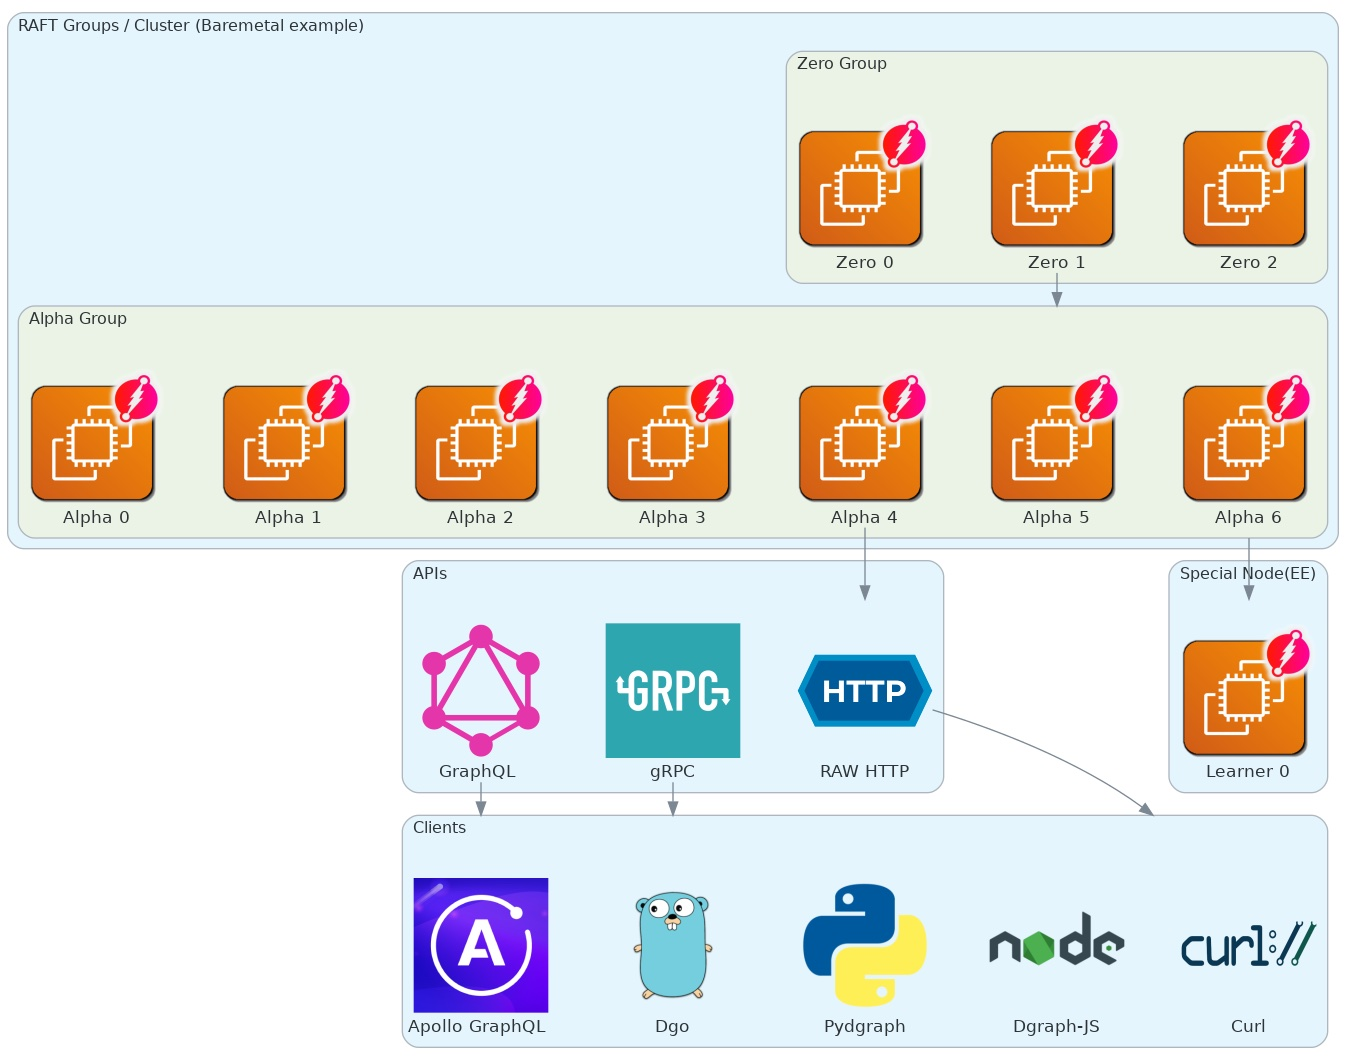
\includegraphics[width=1\textwidth]{Figures/background/dgraph-architecture.jpg}
    \caption{The architecture of a Dgraph cluster with three Zeros and seven Alphas. Taken from Dgraph official documentation.}
    \label{fig:dgraph-architecture}
\end{figure}

Data in Dgraph is stored using the concept of \textit{posting list}. In Dgraph, the unit of data is stored as a composition of three values: \lstinline{<subject> <predicate> <object>}. Every node receives an unique integer id used as the subject. So, for example, a node representing a person with \textit{uid} 1 and name "John" is stored as: \lstinline{<1> <name> <John>}. The actual storage is done by \textit{Badger}, a key-value database. Each unique \lstinline{<subject> <predicate>} is stored as a key with the list of corresponding \lstinline{<object>} as values. So, to complete the example, the person would be stored in the underlying key-value DB as \lstinline{key: <name, 0x1>} and \lstinline{value: <"John">}. Each value is a posting and is stored together with other values sharing the same subject and predicate, effectively forming a posting list.

Sharding in Dgraph is based on \textit{tablets}: a tablet can not be split into multiple servers. A tablet groups data based on predicates. So, reusing the previous example, all the values of the predicate \lstinline{name} form a tablet and so are stored in the same server. Having all the same predicates stored in a single machine allows to perform faster queries since the data to filter is all in one place and there is no need to perform network calls.

Indexes are implemented using the same concept of posting lists. The only difference is that indices are stored using \lstinline{<predicate, token>} as keys instead of \lstinline{<predicate, subject>}. Token is the piece of indexed data and depends on the type. For example, supposing a string \lstinline{"Davide Aimar"} must be indexed using the \textit{term} index, two posting lists will be defined: one with \lstinline{key: <name,"Davide">} and one with \lstinline{key: <name,"Aimar">} containing as values the references to all the uids that have that word in the name.



